\documentclass[11pt,a4paper]{article}
\usepackage[margin=2.3cm]{geometry}
\usepackage{amsmath,amssymb}
\usepackage{graphicx}
\usepackage{booktabs}
\usepackage{siunitx}
\usepackage{hyperref}
\usepackage[font=small]{caption}
\graphicspath{{figures/}}

\title{First- versus second-order mimetic velocity reconstruction\\
       in \texttt{wrf\_ftle}: where the FTLE differs and why}
\author{pv\_ftle --- branch \texttt{2ndorder}}
\date{\today}

\begin{document}
\maketitle

\begin{abstract}
The first-order (lowest-order Raviart--Thomas) and second-order ($Q_{2,1,1}$)
velocity reconstructions of \texttt{wrf\_ftle} were compared on WRF output over
the Transantarctic Mountains and the Ross Ice Shelf ($2.3\times10^6$ seeds,
$T=\SI{-1}{h}$). Over most of the domain the two FTLE fields agree closely
(median difference 2\% of the FTLE scale) and the differences are unbiased,
largest along sharp FTLE ridges. The exception is a predictable, systematic
first-order artefact: in cells into which the (time-reversed) vertical flow
converges, both seeds bounding the cell are drawn into the same layer, where
the first-order wind is constant with height, so they do not separate and the
first-order FTLE collapses. This affects the ground layer most (first-order FTLE
25\% lower on average, holes in 15\% of its cells) and the thick upper layers.
The differences between the orders are 100--1000 times larger than the
time-stepping error, so they come from the reconstruction. Coarsening the data
by 2 and 4 shows the difference between the orders shrinking roughly in
proportion to the grid spacing, and the second-order FTLE changing about three
times less than the first-order one under coarsening: the evidence points to
both converging to the same field, with the first-order error dominating at
WRF's native \SI{3.3}{km} resolution.
\end{abstract}

\section{Introduction}

\texttt{wrf\_ftle} advects particles in index space $(p,q,r)=(i+\xi,\,j+\eta,\,k+\zeta)$
with a mimetic velocity reconstruction built from the WRF face fluxes, and
computes the finite-time Lyapunov exponent (FTLE) from the flow map.
Two reconstructions are available (\texttt{--order 1|2}).
This report compares them on WRF output over the Ross Ice Shelf and the
Transantarctic Mountains, asking three questions:
\begin{enumerate}
  \item Where do first- and second-order FTLE fields differ?
  \item Are the differences predictable from properties of the flow or grid?
  \item Do the two converge to the same FTLE field as the grid is refined?
\end{enumerate}

\section{The two reconstructions}

In a cell, the velocity in index space is
$\dot\xi = F_\xi/J$ (likewise for $\eta,\zeta$), where $J$ is the Jacobian of
the trilinear map and $F_\xi$ the flux density through surfaces of constant $\xi$.
The face data are the face-mean normal velocity $w=\phi/A$ (flux over area)
and the face area $A$.

\paragraph{Order 1} (lowest-order Raviart--Thomas): $F_\xi$ varies linearly
between the two $\xi$-faces of the cell and is constant over each face,
\begin{equation}
  F_\xi = (1-\xi)\,A_0w_0 + \xi\,A_1w_1 .
\end{equation}
The normal component is continuous across faces, but the tangential
components are piecewise constant: they \emph{jump} across every face. In
particular, the horizontal wind is constant with height inside each layer.

\paragraph{Order 2} ($Q_{2,1,1}$): $F_\xi$ is quadratic between the faces and
linear along each face,
\begin{equation}
  F_\xi = (1-\xi)\,A_0\bigl[w_0+s^{(0)}_\eta(\eta-\tfrac12)+s^{(0)}_\zeta(\zeta-\tfrac12)\bigr]
        + \xi\,A_1\bigl[w_1+s^{(1)}_\eta(\eta-\tfrac12)+s^{(1)}_\zeta(\zeta-\tfrac12)\bigr]
        + \tfrac12\bar A\,c\,\xi(\xi-1),
\end{equation}
where the tangential slopes $s$ are central differences of $w$ over the
neighbouring faces (one-sided at the domain edge) and $c$ is the mean second
difference of $w$ across the cell's two faces. The slope terms integrate to
zero over each face and the quadratic term vanishes on both faces, so every
face carries exactly its WRF flux, and the ground and model lid remain
impermeable. Differencing $w$ rather than $\phi$ keeps a constant wind exact on
stretched layers. On box grids, order 2 reproduces a linear wind to round-off
and makes all velocity components continuous across faces
(\texttt{tests/test\_wrf\_reconstruction.py}). It costs about $2.3\times$ the
first-order RK4 time.

\section{Data and method}

\paragraph{Data.} WRF output \texttt{wrf\_f005.nc} (polar stereographic,
$\Delta x=\SI{3.33}{km}$, 60 terrain-following layers, lowest layer
$\approx\SI{25}{m}$ thick), with \texttt{wrf\_f004.nc} for the time-dependent case.

\begin{figure}[t]
  \centering
  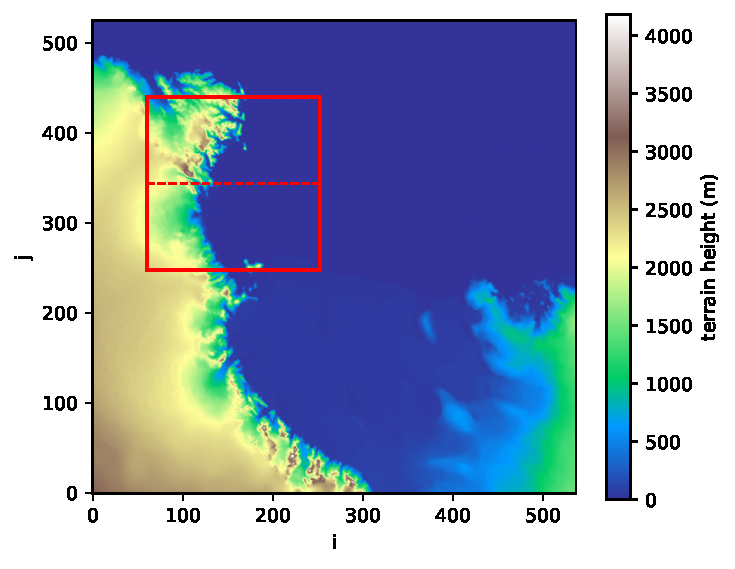
\includegraphics[width=0.55\textwidth]{region}
  \caption{Terrain height of the WRF domain, the study window (red box) and
  the cross-section of Fig.~\ref{fig:section} (dashed).}
  \label{fig:region}
\end{figure}

\paragraph{Study window.} $192\times192$ columns, $i=60$--$252$, $j=248$--$440$
(Fig.~\ref{fig:region}): East Antarctic plateau, the Transantarctic Mountains
(slopes above 3\% in 15\% of the window) and the flat Ross Ice Shelf (53\% of
the window below \SI{10}{m}).
Seeds are placed at every cell corner of the window on all 61 levels
($2.27\times10^6$ seeds); particles move over the whole domain.

\paragraph{Integration.} Backward in time, $T=\SI{-3600}{s}$, frozen wind from
\texttt{wrf\_f005} unless stated otherwise, RK4 with CFL 0.5 (509 steps),
using the C++ integrator (double precision). FTLE is the cell-centred 3-D FTLE
of \texttt{wrf\_ftle}. Differences are reported relative to the FTLE scale
$S=\SI{1.40e-3}{s^{-1}}$, the 99th percentile of the order-2 FTLE.
Approximate heights above ground of the levels quoted below: level 0
\SI{13}{m}, 1 \SI{45}{m}, 3 \SI{145}{m}, 5 \SI{290}{m}, 10 \SI{880}{m},
20 \SI{3.1}{km}, 30 \SI{7.0}{km}, 40 \SI{13.6}{km}, 55 \SI{27}{km}.

\paragraph{Separating the effects.} The two orders are compared with the
same seeds, time step and grid, so any difference comes from the reconstruction.
A time-step series (CFL 1, 0.5, 0.25) checks that time-stepping error is
small compared with the order difference.

\paragraph{Grid refinement.} WRF cannot be refined, so the data were
\emph{coarsened} by $c=2$ and $4$: every $c$-th corner is kept and fine face
fluxes are summed over $c\times c$ sub-faces (with their areas). This conserves
the flux through every coarse face exactly (checked to $10^{-15}$), so the
coarse grids are nested, flux-consistent versions of the fine one. A common
set of seeds (every 4th corner and level, $49\times49\times16$) is tracked on
all three grids with both orders and the same time step, and the final
positions and FTLE are compared. If both orders converge to the same limit,
their difference must shrink as the grid is refined.

\section{Results}

\subsection{Overall size of the differences}

Over all $2.2\times10^6$ cells, $|\mathrm{FTLE}_2-\mathrm{FTLE}_1|/S$ has a
median of 2.2\%, a 95th percentile of 15\% and a 99th percentile of 33\%;
72\% of cells differ by more than 1\% and 10\% by more than 10\%.

The time step is not the cause (Fig.~\ref{fig:timestep}). Halving CFL from 0.5
to 0.25 changes the FTLE by a median of $4.0\times10^{-5}S$ at order 1 and
$6.6\times10^{-6}S$ at order 2 (95th percentiles $7.6\times10^{-4}S$ and
$1.5\times10^{-4}S$), while the two orders differ by a median of $2.1\times10^{-2}S$
at the same CFL. The order difference is therefore a spatial-discretisation
effect, 100--1000 times larger than the time-stepping error; order 2 is also
about five times less sensitive to the time step, consistent with its smoother
velocity field.

\begin{figure}[t]
  \centering
  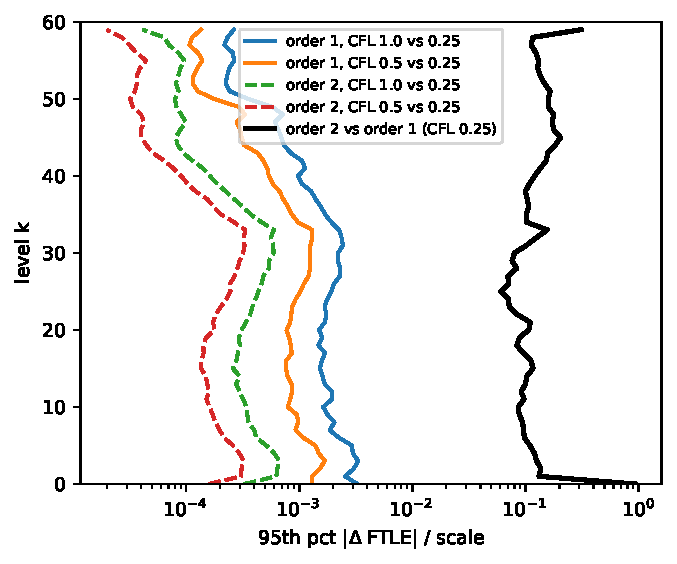
\includegraphics[width=0.48\textwidth]{timestep}
  \caption{95th percentile, per level, of the FTLE change between CFL 1 or 0.5
  and CFL 0.25 for each order, against the difference between the orders
  (black).}
  \label{fig:timestep}
\end{figure}

\subsection{Where the differences occur}

\begin{figure}[p]
  \centering
  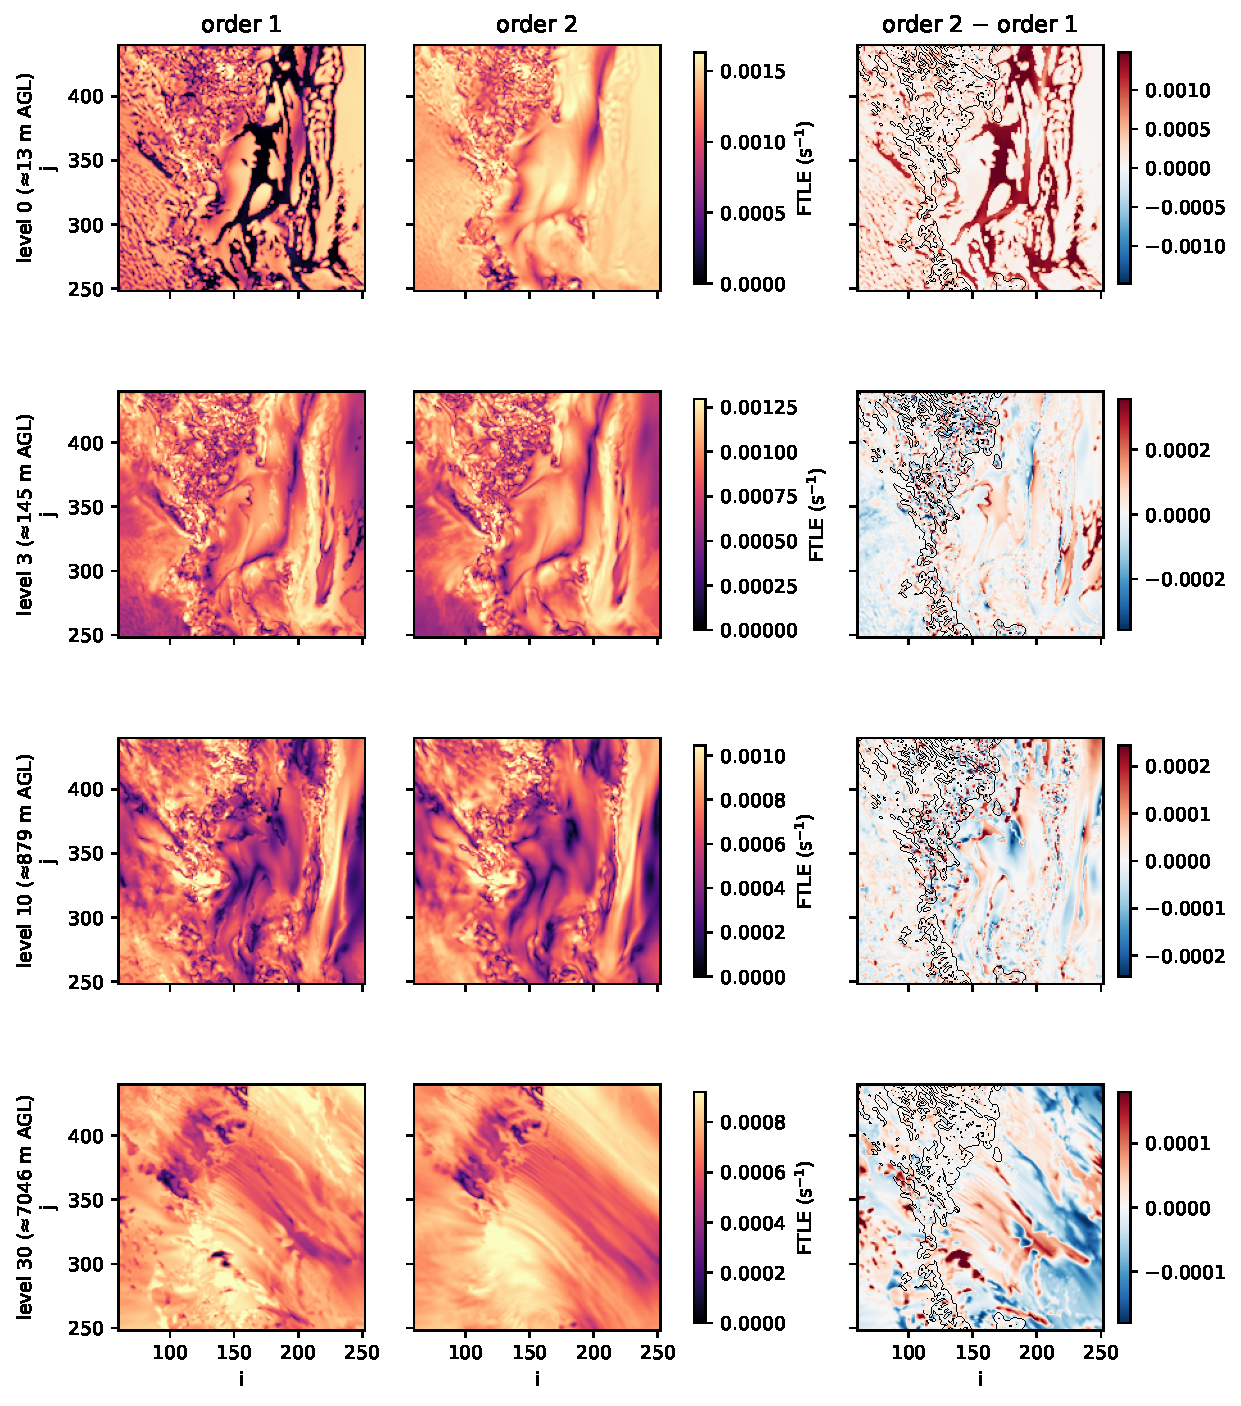
\includegraphics[width=0.95\textwidth]{maps}
  \caption{FTLE of order 1 (left) and order 2 (centre) and their difference
  (right) at four levels. Black contours on the difference maps: terrain
  slope 3\%.}
  \label{fig:maps}
\end{figure}

\begin{figure}[t]
  \centering
  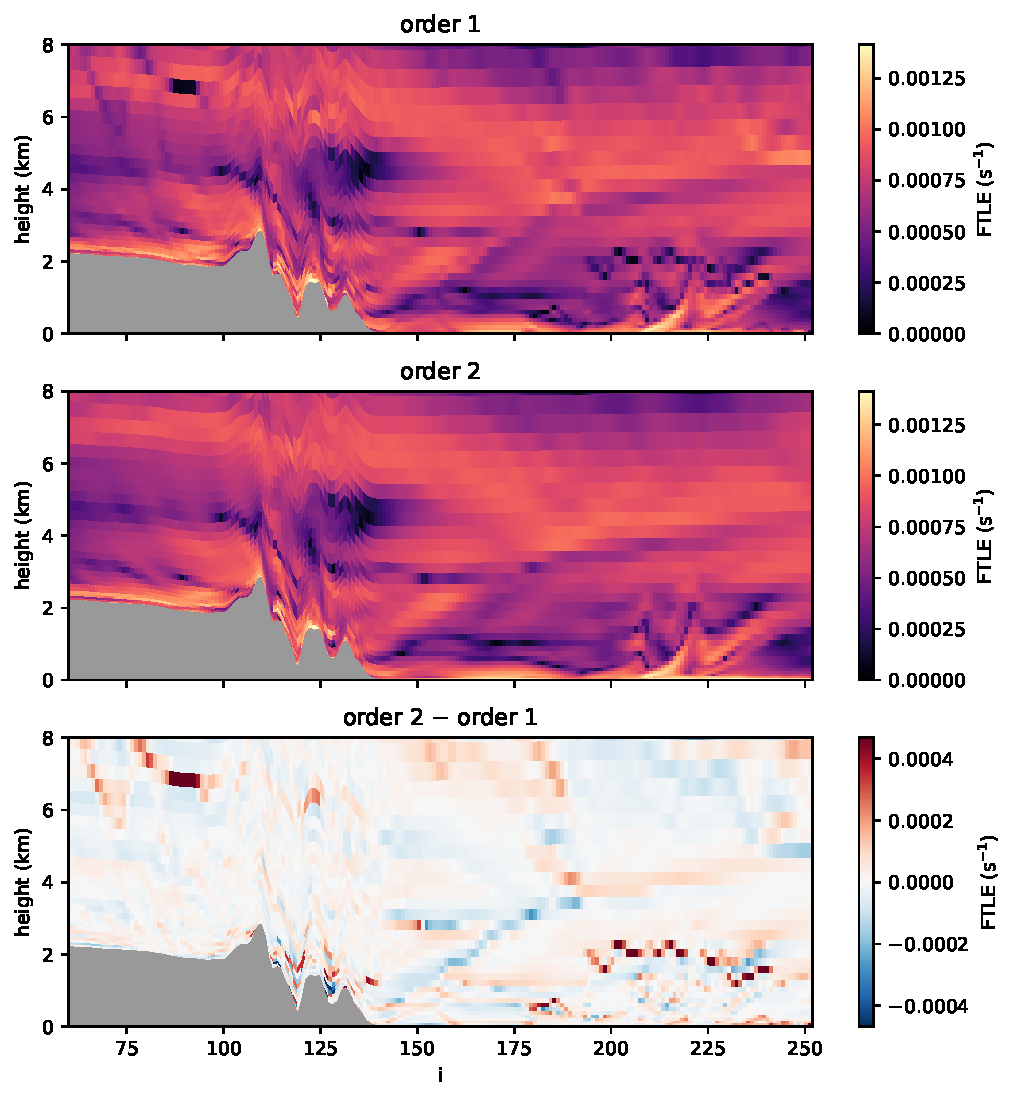
\includegraphics[width=0.8\textwidth]{section}
  \caption{Cross-section along $j=344$ from the plateau (left) over the
  mountains to the ice shelf (right), lowest \SI{8}{km}. Grey: terrain.}
  \label{fig:section}
\end{figure}

\begin{figure}[t]
  \centering
  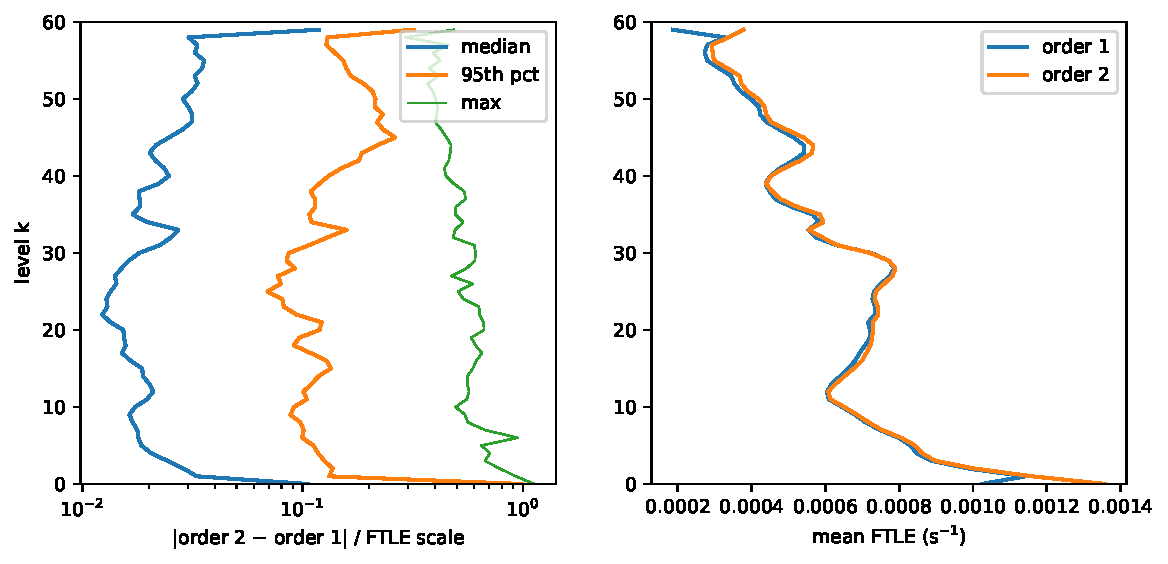
\includegraphics[width=0.85\textwidth]{by_level}
  \caption{Left: distribution of $|\mathrm{FTLE}_2-\mathrm{FTLE}_1|/S$ per
  level. Right: mean FTLE per level for both orders.}
  \label{fig:bylevel}
\end{figure}

Figures~\ref{fig:maps}--\ref{fig:bylevel} show three regimes.

\paragraph{The ground layer (level 0).} The largest and only strongly
systematic differences. The first-order field has sharp-edged ``holes'' of
near-zero FTLE, mostly over the flat ice shelf (Fig.~\ref{fig:maps}, top row,
and the near-surface blocks in Fig.~\ref{fig:section}) that are absent at
order 2. The median difference is 10.5\% of $S$ and the 95th percentile 99\%;
the mean first-order FTLE of the layer is 25\% lower
(\num{1.02e-3} versus \SI{1.36e-3}{s^{-1}}, Fig.~\ref{fig:bylevel}, right).

\paragraph{The free atmosphere (levels 1--40).} Small and unbiased: median
differences 1.5--3.3\% of $S$, mean FTLE per level equal to within about 1\%.
The differences are fine-scale and of both signs, lying along the edges of
FTLE filaments (levels 3 and 10 in Fig.~\ref{fig:maps}); aloft (level 30,
\SI{7}{km}) they become smooth, larger-scale patterns of about 10\% of $S$,
where the layers are several hundred metres thick and the first-order wind
is constant over that depth.

\paragraph{The thick upper layers (levels $\gtrsim 40$, above \SI{14}{km}).}
Median differences rise again to 4--6\% and first-order holes reappear
(Fig.~\ref{fig:predictors}, left).

\subsection{A predictable pattern: trapped seeds}

The holes have a simple cause. At order 1 the horizontal wind is constant with
height inside a layer, and a seed lying exactly on a level is assigned to the
layer above it. Integrating backward in time, a seed on a level moves down
where $W>0$ on that level and up where $W\le0$. In a cell with
$W\le0$ on its bottom face and $W>0$ on its top face (a layer into which the
time-reversed vertical flow converges), the seed on the bottom face stays in
the cell and the seed on the top face drifts down into it: both then move with
the \emph{same} first-order wind and do not separate vertically, so the
first-order FTLE collapses. At order 2 the wind varies linearly with height
inside the layer and the two seeds keep separating. At the ground $W=0$, so
the condition reduces to $W>0$ on level 1. For forward integration the signs
flip ($W\ge0$ below, $W<0$ above).

\begin{figure}[t]
  \centering
  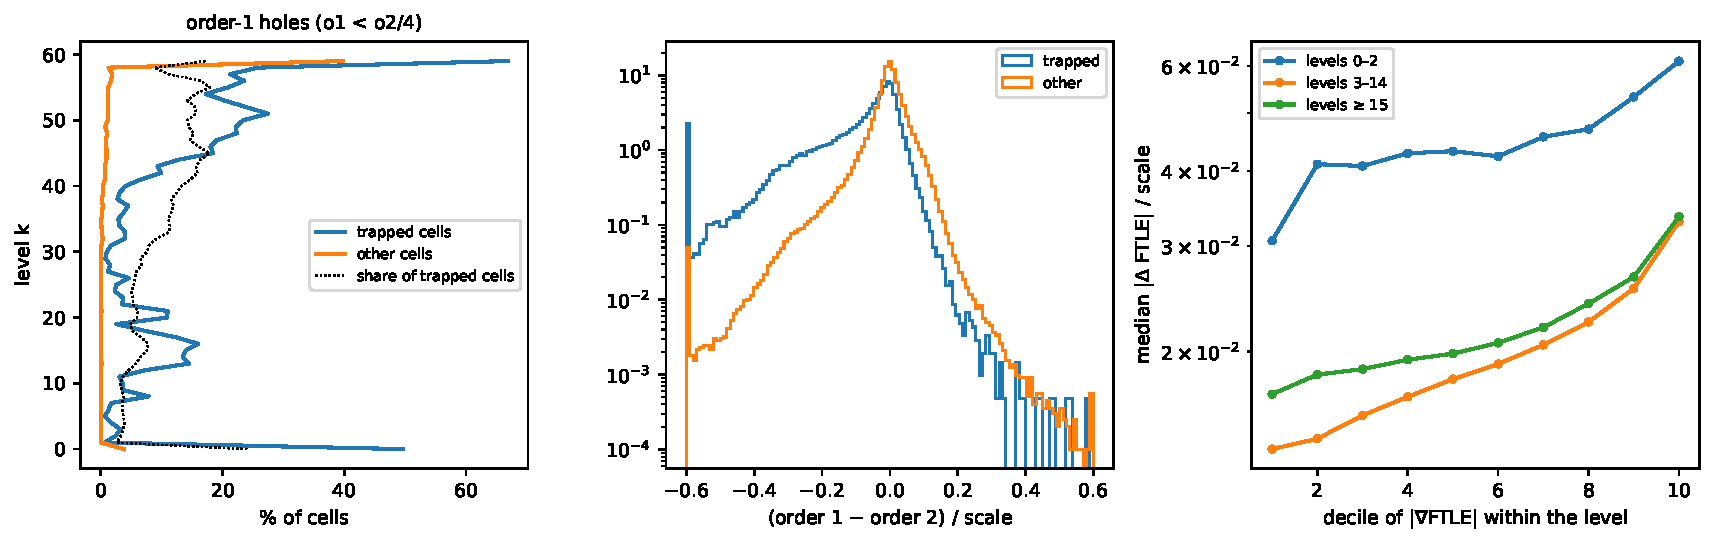
\includegraphics[width=\textwidth]{predictors}
  \caption{Left: percentage of cells with a first-order hole
  ($\mathrm{FTLE}_1<\mathrm{FTLE}_2/4$) per level, for trapped cells
  ($W\le0$ below, $W>0$ above) and all other cells; dotted: share of trapped
  cells. Centre: distribution of $(\mathrm{FTLE}_1-\mathrm{FTLE}_2)/S$ for
  trapped and other cells. Right: median $|\Delta\mathrm{FTLE}|/S$ against the
  decile of the FTLE gradient within each level.}
  \label{fig:predictors}
\end{figure}

\begin{table}[t]
  \centering
  \caption{First-order holes ($\mathrm{FTLE}_1<\mathrm{FTLE}_2/4$) in trapped
  cells and in all other cells; $F_1,F_2$: first- and second-order FTLE.}
  \label{tab:trapped}
  \small
  \begin{tabular}{lrrrr}
    \toprule
     & cells & hole rate & median $F_1/F_2$ & mean $(F_1-F_2)/S$ \\
    \midrule
    trapped cells & 9.6\% & 15.2\% & 0.89 & $-10.1\%$ \\
    other cells   & 90.4\% & 1.0\% & 1.00 & $-0.5\%$ \\
    \midrule
    level 0, trapped  & 24\% & 50\% & 0.27 & \\
    level 55, trapped & 18\% & 21\% & 0.63 & \\
    \bottomrule
  \end{tabular}
\end{table}

Table~\ref{tab:trapped} confirms the rule: trapped cells are 9.6\% of all cells
but contain 61\% of the holes, with a hole rate of 15\% against 1\% elsewhere,
and carry the systematic negative bias of order 1. The effect is strongest in
the ground layer (half of its trapped cells are holes) and in the thick upper
layers; in the thin layers of the lower and middle troposphere a trapped seed
soon leaves the layer and the effect is weak (hole rates below 1\% at levels
1--5). At level 0, the mean bias is $-40\%$ of $S$ where $W>0$ on level 1 and
$-11\%$ where $W\le0$.

The size of the wind jump between layers does \emph{not} predict the
differences (rank correlation $-0.04$ within trapped cells), so the effect
depends on the vertical motion, not on the shear.

Away from trapped cells the differences are largest where the FTLE field is
sharpest (Fig.~\ref{fig:predictors}, right): from the smoothest to the sharpest
decile of the FTLE gradient the median difference rises from 1.4\% to 3.3\%
(levels 3--14) and from 3.1\% to 6.1\% (levels 0--2), as expected if the
reconstruction mainly shifts ridges slightly. Near the ground the differences
also grow with terrain slope, from 4.2\% (slope below 0.5\%) to 6.2\% (slope
above 10\%) of $S$ in levels 0--2.

\paragraph{Time-dependent wind.} With the wind interpolated between
\texttt{wrf\_f004} and \texttt{wrf\_f005}, the statistics are almost identical
(median 2.1\%, 95th percentile 14\%, level 0 median 10.9\%; Fig.~\ref{fig:timedep}).

\begin{figure}[t]
  \centering
  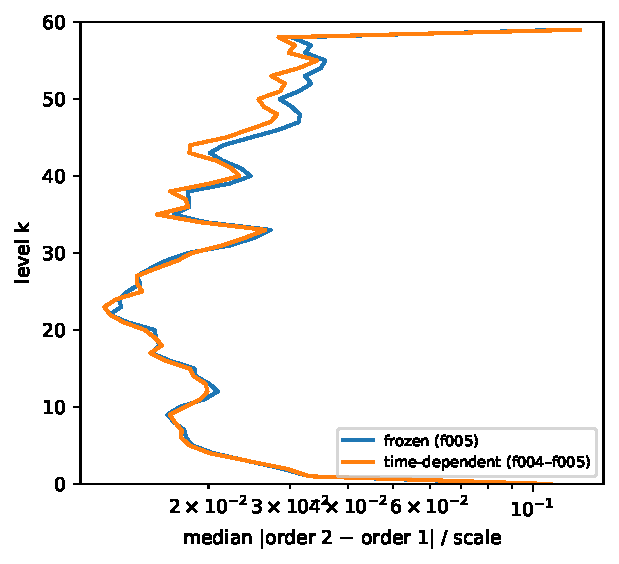
\includegraphics[width=0.45\textwidth]{timedep}
  \caption{Median $|\mathrm{FTLE}_2-\mathrm{FTLE}_1|/S$ per level, frozen
  versus time-dependent wind.}
  \label{fig:timedep}
\end{figure}

\subsection{Do the two orders converge to the same field?}

\begin{figure}[t]
  \centering
  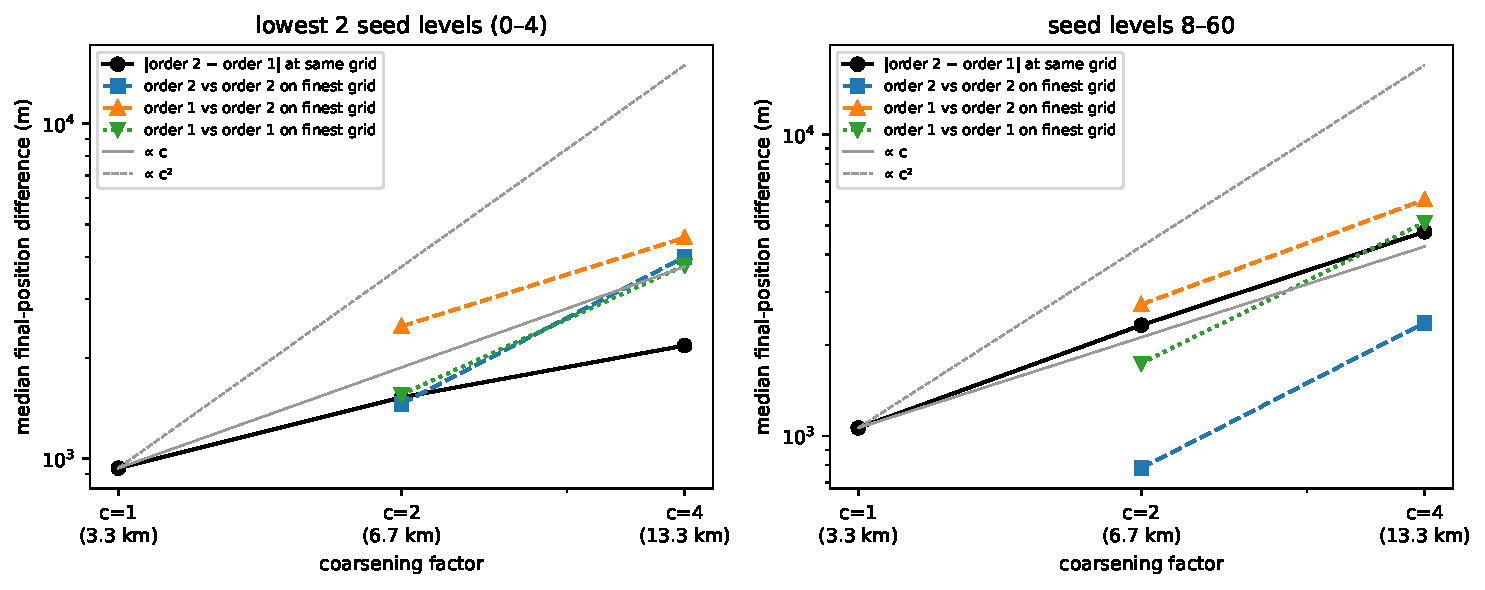
\includegraphics[width=\textwidth]{resolution}
  \caption{Median distance between final particle positions on the common
  seed lattice for grids coarsened by $c=1,2,4$: between the orders on the same
  grid (black), and of each order against the finest grid. Left: the two
  lowest seed levels; right: seed levels 8--60. Grey: slopes $\propto c$ and
  $\propto c^2$.}
  \label{fig:resolution}
\end{figure}

\begin{figure}[t]
  \centering
  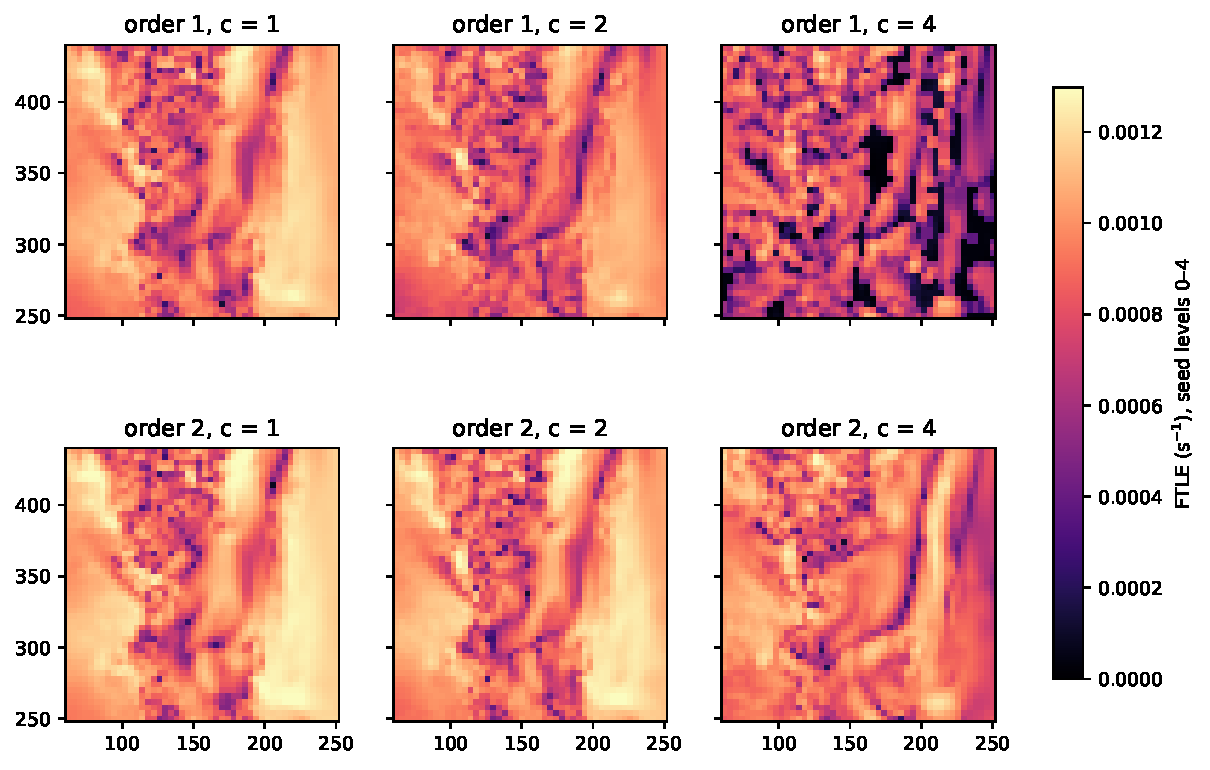
\includegraphics[width=0.85\textwidth]{resolution_maps}
  \caption{FTLE of the lowest cell layer of the common seed lattice (seed
  levels 0--4) on the native ($c=1$) and coarsened ($c=2,4$) grids.}
  \label{fig:resmaps}
\end{figure}

\begin{table}[t]
  \centering
  \caption{Median FTLE differences on the common seed lattice, relative to
  $S$, for grids coarsened by $c$ (\SI{3.3}{km}, \SI{6.7}{km}, \SI{13.3}{km}).}
  \label{tab:resolution}
  \begin{tabular}{lrrr}
    \toprule
     & $c=1$ & $c=2$ & $c=4$ \\
    \midrule
    order 2 vs order 1, same grid        & 1.2\% & 2.8\% & 4.9\% \\
    order 2 vs order 2 at $c=1$          & ---   & 0.7\% & 3.0\% \\
    order 1 vs order 1 at $c=1$          & ---   & 2.0\% & 5.8\% \\
    \bottomrule
  \end{tabular}
\end{table}

The difference between the orders shrinks steadily as the grid is refined
(Fig.~\ref{fig:resolution}, Table~\ref{tab:resolution}). For final positions
above the lowest seed levels it falls from \SI{4.8}{km} ($c=4$) to
\SI{2.3}{km} ($c=2$) to \SI{1.1}{km} ($c=1$), about a halving per refinement
(median displacement \SI{26}{km}); for the FTLE it falls from 4.9\% to 2.8\% to
1.2\% of $S$. Near the ground it shrinks more slowly (\SI{2.2}{km},
\SI{1.5}{km}, \SI{0.9}{km}), where the trapping artefact of order 1 depends on
the vertical motion and not on the grid spacing alone.

Each order also converges towards its own finest-grid result. Second-order
FTLE changes about three times less than first-order FTLE between $c=2$ and
$c=1$ (0.7\% versus 2.0\%), and the second-order field at \SI{6.7}{km} is
closer to the second-order field at \SI{3.3}{km} than the two orders are to
each other at \SI{3.3}{km} (0.7\% versus 1.2\%). Visually
(Fig.~\ref{fig:resmaps}), order 2 keeps the structure of the ground-layer FTLE
down to $c=4$, while order 1 develops large holes as the layers thicken.

With only three resolutions, and the native WRF grid as the finest, these
figures are estimates of the trend, not a proof of convergence. They are,
however, consistent with both reconstructions converging to the same FTLE
field, with an inter-order difference that decreases roughly in proportion to
the grid spacing --- the signature of the first-order error dominating it.

\section{Conclusions}

\begin{enumerate}
  \item \textbf{Where.} Over most of the atmosphere the two orders give nearly
  the same FTLE: median differences of 1.5--3\% of the FTLE scale, unbiased,
  concentrated along sharp FTLE ridges. Large, systematic differences occur in
  the ground layer (first-order FTLE 25\% lower on average) and in the thick
  upper layers above about \SI{14}{km}.
  \item \textbf{Predictable pattern.} The systematic differences are a
  first-order artefact with a simple rule: in cells into which the
  (time-reversed) vertical flow converges --- $W\le0$ on the bottom face and
  $W>0$ on the top face for backward FTLE --- both bounding seeds share one
  layer's constant first-order wind and the FTLE collapses. These cells hold
  61\% of the first-order holes. Order 2 avoids this because its wind varies
  linearly with height inside each layer.
  \item \textbf{Convergence.} The difference between the orders shrinks
  roughly in proportion to the grid spacing under coarsening, and order 2 is
  about three times less sensitive to resolution, so the evidence is that both
  converge to the same FTLE field, with order 1's error dominating at WRF's
  native resolution. At \SI{3.3}{km} the remaining median difference is about
  1--2\%, but individual first-order cells can be wrong by 100\%.
  \item \textbf{Recommendation.} Use order 2 (the default). Treat first-order
  FTLE in the lowest layer and in thick upper layers with caution, especially
  where the vertical velocity changes sign across a layer. The extra cost of
  order 2 (about $2.3\times$ the RK4 time) is small compared with the
  accuracy gained.
\end{enumerate}

\appendix
\section{Reproducing}
\begin{verbatim}
python scripts/order_study_run.py WRF_DIR DATA_DIR
python scripts/order_study_figures.py DATA_DIR WRF_DIR \
       report/order2/figures
cd report/order2 && latexmk -pdf order2.tex
\end{verbatim}
{\sloppy
\texttt{WRF\_DIR} holds \texttt{wrf\_f004.nc} and \texttt{wrf\_f005.nc}.
Numbers quoted in the text are in \texttt{figures/stats.json}.\par}

\end{document}
